\section{Algorithm description}\label{implementacion}
A motion capture system with the necessary characteristics to achieve the objective of this project must implement four general blocks: 
\emph{calibration}, \emph{segmentation}, \emph{reconstruction} and \emph{tracking}. Figure \ref{bloquesSist} shows a scheme of the system to be implemented, every green block indicates a stage output, being at the same time next block input.
%\vspace{-0.6cm}
\begin{figure}[ht!]
\centering
\hspace{-0.5cm}
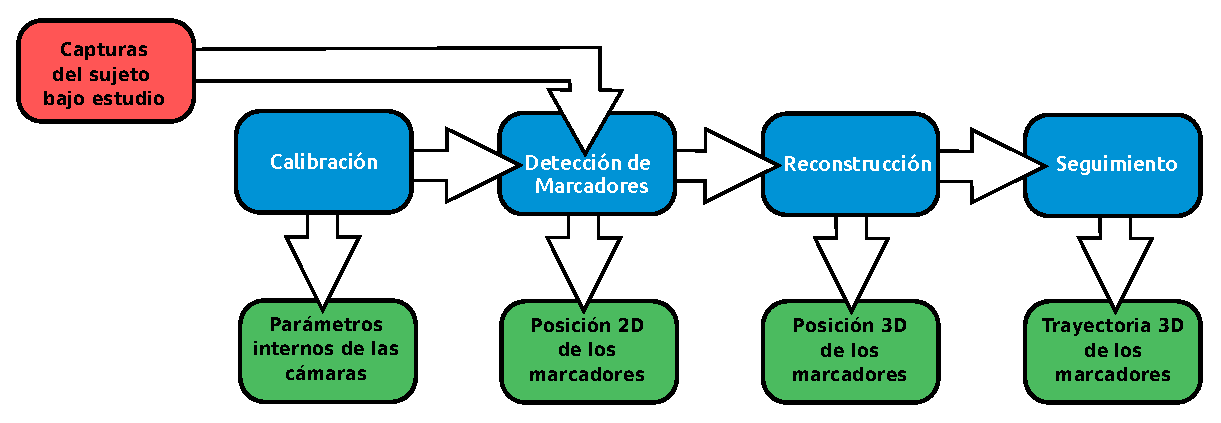
\includegraphics[scale=0.4]{imagenes/Sistema_completo/Diagrama_de_bloques.eps}
\caption{Block diagram of complete system.}
\label{bloquesSist}
\end{figure}
%\vspace{-0.7cm}

It is important to highlight the independence between blocks, allowing to modify or easily optimize the system in future stages.
